\documentclass[conference]{IEEEtran}
\IEEEoverridecommandlockouts
% The preceding line is only needed to identify funding in the first footnote. If that is unneeded, please comment it out.
\usepackage{cite}
\usepackage{amsmath,amssymb,amsfonts}
\usepackage{algorithmic}
\usepackage{graphicx}
\usepackage{float}
\usepackage{textcomp}
\usepackage{xcolor}
\usepackage{hyperref}
\usepackage{url}

\def\BibTeX{{\rm B\kern-.05em{\sc i\kern-.025em b}\kern-.08em
    T\kern-.1667em\lower.7ex\hbox{E}\kern-.125emX}}
\begin{document}

\title{Rumor Verification using Evidence from Authorities\\
% {\footnotesize \textsuperscript{*}Note: Sub-titles are not captured in Xplore and
% should not be used}
% \thanks{Identify applicable funding agency here. If none, delete this.}
}

\author{Perambuduri Srikaran\\
AI20BTECH11018\\
% For a paper whose authors are all at the same institution,
% omit the following lines up until the closing ``}''.
% Additional authors and addresses can be added with ``\and'',
% just like the second author.
% To save space, use either the email address or home page, not both
\and
Shambhu Prasad Kavir\\
CS20BTECH11045\\
\and
Taha Adeel Mohammed\\
CS20BTECH11052\\
}

\maketitle


\begin{abstract}
The spread of rumors on social media platforms like Twitter can have significant real-world consequences. This work addresses the critical task of rumor verification.

To solve this problem, we design a two-stage pipeline. In the first stage, we use ColBERT for information retrieval to fetch the top-$k$ similar tweets for a given rumor. In the second stage, we use MISTRAL to appropriately classify the rumor and retrieve the top-5 evidences using the tweets retrieved.
\end{abstract}

% \begin{IEEEkeywords}
% component, formatting, style, styling, insert
% \end{IEEEkeywords}

\section{Introduction}
With the huge amount of information and misinformation available and being generated on social media platforms, it is important to verify the credibility of the information that is shared via these platforms. There also happen to be relatively trustworthy accounts managed by the authorities, which can be used as a source of evidence for the validity of the buzz or rumor being spread. In this project, we aim to do rumor verification using evidence from the authorities timelines. 

\section{Problem Statement}
\subsection{Aim}
Given a rumor expressed in a tweet and a set of authorities(one or more Twitter accounts) for that rumor, represented by a list of tweets from their timelines during the period surrounding the rumor, the system should retrieve up to 5 evidence tweets from those timelines, and determine if the rumor is supported (true), refuted (false) or unverifiable (in case not enough evidence exists in the given tweets) according to the evidence. \cite{problem-statement}
\subsection{Dataset}
\begin{figure}[htp]
    \centering
    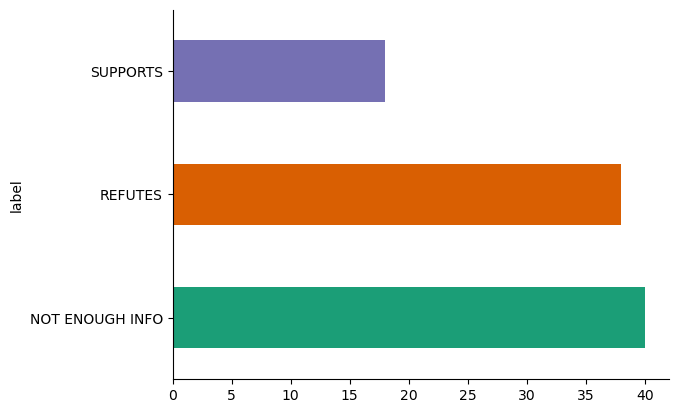
\includegraphics[width=\columnwidth]{images/dataser.png}
    \caption{Dataset statitics}
    \label{fig:es}
\end{figure} 
The dataset is composed of two files:- \texttt{Task 5--Arabic-v1.0 [2024/02/14]} and \texttt{Task 5--English-v1.0 [2024/02/14]}, with the former containing Arabic data and the latter English.\cite{input_data} \\
Figure-1 shows the distribution of the data points based on their labels for the Arabic dataset. We note that there are 20 rumors with the label SUPPORTS, 37 with the label REFUTES and 40 with the label NOT ENOUGH INFO.\\
Input - Each data point in the dataset has the following entries:-
\begin{itemize}
    \item \textbf{id} - unique ID of the rumor
    \item \textbf{rumor} - rumor tweet text
    \item \textbf{label} - SUPPORTS, REFUTES or NOT ENOUGH INFO
    \item \textbf{timeline} - authorities timeline associated with the rumor; each authority tweet is represented by authority Twitter account link, authority tweet ID, authority tweet text
    \item \textbf{evidence} - authorities evidence tweets represented by authority Twitter account link, authority tweet ID, authority tweet text  
\end{itemize}
Output -
\begin{itemize}
    \item \textbf{Evidence Retrieval} - For each rumor, upto 5 evidence authority tweets are retrieved
    \item \textbf{Rumor Verification} - Given a rumor, along with upto 5 evidence tweets, a label is predicted (SUPPORTS, REFUTES, NOT ENOUGH INFO) 
    
\end{itemize}

\section{Literature Review}
% Put from the first presentation
\subsection{Related Work}
The Fact Extraction and VERification \cite{fever} (FEVER) Shared Task challenged participants to classify whether human-written factoid claims could be supported or refuted using evidence retrieved from Wikipedia. The task recieved 23 entries, with the best one having a 64.21\% accuracy. 

Factify \cite{factify} is a multi-modal fact verification dataset and shared task consisting of 50,000 data points covering new articles along with images from India and the US. It encouraged researchers to focus on the multi modality along with the fact verification.

Previous work by Mohna et. al. \cite{chat-gpt-study} did a study on the performance of ChatGPT on the fact verification task. From the study, they found that most of the errors by chatGPT were due to incorrect logical reasoning and contextual misunderstanding of the claim.

The baseline model used by the task organizers is using Kernel Graph Attention Network (KGAT) \cite{kgat}, which is a model that conducts fine-grained  fact verification with kernel-based attentions.

The authors of the task, Fatima Haouari et. al. also have a series of papers for rumor verification on Twitter. In the first paper \cite{fh1}, they focus on finding authorities for rumor verification, along with information processing and management. Then \cite{fh2} they focus on detecting the authority stances in arabic tweets, along with advancements in information retrieval. The third paper \cite{fh3} focuses on social network analysis and mining, generating the dataset for rumor verification.

\subsection{Information Retrieval}
\subsubsection{Elastic Search}
Elastic search\cite{elastic-search} is a well-known information retrieval/search engine based on Apache Lucine that is known for its speed and accuracy. It is a statistical model based on inverted indexing, hashing and internal tree like structuring of the data, allowing for its very fast search capabilities. It also employs different ranking algorithms like BM25 to rank the documents based on their relevance to the query. It also supports hybrid retrieval, i.e lexical + semantic retrieval to improve the search accuracy.
\begin{figure}[htp]
    \centering
    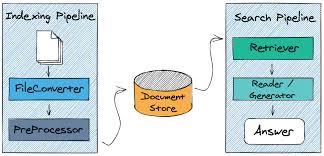
\includegraphics[width=\columnwidth]{images/ES.png}
    \caption{Working of Elastic Search\cite{es-image}}
    \label{fig:es}
\end{figure} 

\subsubsection{ColBERT}
ColBERT is another information retrieval model, based on transformers, that is good at capturing semantic meanings in its results. It makes use of a pre-trained BERT model to generate encoded representations for both the user query and individual documents within the collection. BERT excellence at capturing semantic meaning in text, aiding ColBERT in grasping the semantic intent and similarity between the queries and documents. 

Instead of directly comparing the query and document encodings, ColBERT employs a two-step approach for efficient retrieval. It first computes the maximum similarity score between each element in the query's encoding and all corresponding elements in each document's encoding. Hence, it can focus its "attention" on the most relevant parts of the document. 

To speed up the retrieval process, ColBERT pre-computes the encodings for all the documents in the collection offline. Hence when a user submits a query, the model only needs to encode the query itself and then compare it against the precomputed document encodings. This allows for very fast queries, making the model scalable and suitable for real time querying.

\begin{figure}[htp]
    \centering
    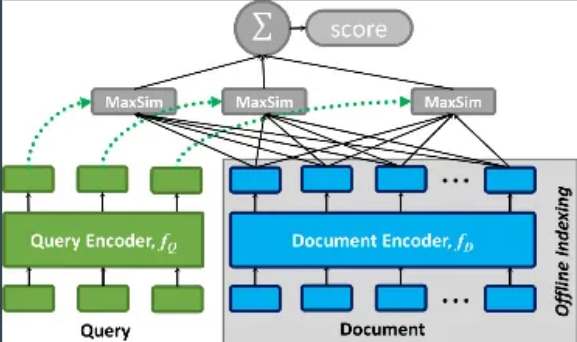
\includegraphics[width=\columnwidth]{images/colbert.png}
    \caption{Architecture of ColBERT \cite{colbert}}
    \label{fig:colbert}
\end{figure}

\subsection{Large Language Models}
\subsubsection{Llama}
Llama is an accessible, open-source LLM that is based on standard transfomer architecture. It uses RMSNorm for pre-normalization and uses SWiGLU activation function. It allows a context window of upto 4096 tokens, and utilizes group query attention for efficiency. 

\subsubsection{Mistral 7B}
Mistral is series of transformer-based decoder-only models, and one of the most powerful open source LLMs available, perfoming better than its competitors like Llama, and GPT-3 on various benchmarks. The company offers multiple versions of the model, with us opting for the 7B version, which has 7 billion parameters, a good balance between performance and storage and computational costs. It does so using sliding window attention, rolling buffer cache, pre-fill, and chunking. 


\section{Our Approach}

\begin{figure}[htp]
    \centering
    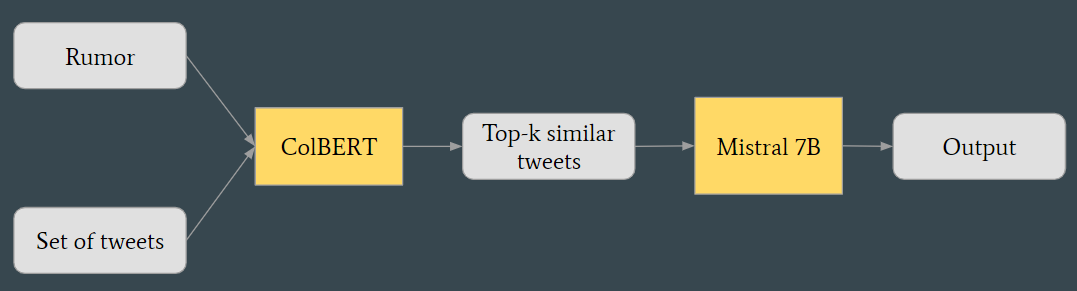
\includegraphics[width=\columnwidth]{images/approach.png}
    \caption{Overall Pipeline of the Approach}
    \label{fig:colbert}
\end{figure}

For our approach, as shown in figure \ref{fig:colbert}, we have a two-stage pipeline. In the first stage, we use ColBERT for information retrieval to fetch the top-$k$ similar tweets for a given rumor. Now having reduced the sample space for the possible evidence tweets, we pass these top-$k$ tweets to the LLM Mistral to classify the rumor and retrieve the top-5 evidences using the tweets retrieved. We claim that the pipeline allows us to accurately perform the rumor verification in a scalable and efficient manner. To further boost our accuracy, we fine-tune our information retrieval model ColBERT using the training data.


\section{Experiments}

\subsection{Experimental Setup}
\subsubsection{Hardware and Software}
The experiments were run on kaggle's cloud platform, using 16GB T4 GPUs. The scripts were written in Python, using the Hugging Face Transformers library for the LLM Mistral, and the ColBERT library for the information retrieval model. The mistrel model weights were downloaded from the Hugging Face model hub, and the ColBERT model was fine-tuned on the training data.\\

\subsubsection{Prompt}
The prompt we used to pass through Mistral to get our final output is as follows:

\texttt{You have to prove the following rumor is supported or refuted by the tweets given. If either of them can be done, just write either SUPPORTS or REFUTES.}

\texttt{If it is not possible to prove, tell NOT ENOUGH INFO.}

\texttt{The output should be in this format. }

\texttt{REFUTES}

\texttt{Pictures from the launch of the vaccination campaign against the \#Coronavirus, starting with the medical and health teams in \#Bethlehem. \#vaccine \#Palestine \#COVID19 https://t.co/vnhGmoZtgC}

\texttt{The Ministry added that the second group that will receive the vaccine is the elderly over the age of 60 and those with chronic diseases, because if they are infected with the virus, they will be more susceptible to serious symptoms. \#vaccine \#modernavaccine \#palestine \#COVID19}

\texttt{[rumor]}

\texttt{To prove it, use the following tweets and see which tweets support or refute the rumor:}

\texttt{Output upto 5 tweets which prove or refute the rumor as it is with the number}

\texttt{[top-k tweets obtained from ColBERT]}

\subsection{Evaluation Metrics}
\begin{itemize}
    \item \textbf{Mean Average Precision - }The Mean Average Precision is calculated by finding the average precision for each class and calculating the average over several classes.
    \begin{align}
        mAP = \frac{1}{N} \sum_{k=1}^{N} AP_k
    \end{align}
    \item \textbf{Recall@K - }It measures the proportion of correctly identified relevant items in the top K recommendations out of the total number of relevant items in the dataset.
    \begin{align}
        Recall(R)_k = \frac{|{r\in R: r \le k}|}{|R|} 
    \end{align}
    \item \textbf{Macro-F1 - }Macro-F1 is computed using the arithmetic mean of all the per-class F1 scores. 
    \begin{align}
        \text{Macro F1 score} = \sum_{i=1}^{n} \frac{F1 Score_i}{n}
    \end{align}
\end{itemize}


\subsection{Results}
\begin{table}[h]
  \centering
  \begin{tabular}{|c|c|c|}
    \hline
    Metric & Our Score & KGAT-Score \\ \hline
    Recall@5  & 0.57 & 0.64 \\
    AP  & 0.52  & 0.59\\
    Macro-F1  & 0.39 & 0.45  \\
    \hline
\end{tabular}
\label{tab:results}
\caption{Scores}
\end{table}
In the above table \ref{tab:results}, we have the scores for the evaluation metrics for our model. We see that the results are compareable to the baseline model \cite{kgat} for the task. 


\section{Future Work}
\begin{itemize}
    \item We want to ensemble ColBERT with Elastic Search to exploit the different ways of retrieval done by both of them.
    \item We can also try out GPT-4 to get better results in the second stage of the pipeline
\end{itemize}


\begin{thebibliography}{00}
\bibitem{problem-statement} \url{https://gitlab.com/checkthat_lab/clef2024-checkthat-lab/-/tree/main/task5?ref_type=heads#task-5-rumor-verification-using-evidence-from-authorities}
\bibitem{input_data} \url{https://gitlab.com/checkthat_lab/clef2024-checkthat-lab/-/tree/main/task5/#input-data-format}
\bibitem{output_data} \url{https://gitlab.com/checkthat_lab/clef2024-checkthat-lab/-/tree/main/task5/#output-data-format}
\bibitem{fever} The Fact Extraction and VERification (FEVER) Shared Task (Thorne et al., EMNLP 2018)
\bibitem{kgat} Fine-grained Fact Verification with Kernel Graph Attention Network (Liu et al., ACL 2020)
\bibitem{chat-gpt-study} An Empirical Study of Using ChatGPT for Fact Verification Task (2023) - Mohna Chakraborty, Adithya Kulkarni, Qi Li. \url{https://arxiv.org/abs/2311.06592}
\bibitem{factify} \url{https://competitions.codalab.org/competitions/35153#learn_the_details-overview}
\bibitem{elastic-search} \url{https://www.elastic.co/guide/en/elasticsearch/reference/current/getting-started.html}
\bibitem{es-image} \url{https://medium.com/@cesarescalia/guide-haystack-deepset-qa-from-a-pdf-d3f83d76d9d2}
\bibitem{colbert} ColBERT: Efficient and Effective Passage Search via Contextualized Late Interaction over BERTn \url{https://arxiv.org/pdf/2004.12832}
\bibitem{fh1} Who can verify this? Finding authorities for rumor verification in Twitter - Fatima Haouari, Tamer Elsayed, Watheq Mansour - Information Processing and Management Volume 60, Issue 4, July 2023
\bibitem{fh2} Detecting Stance of Authorities towards Rumors in Arabic Tweets: A Preliminary Study - Fatima Haouari, Tamer Elsayed - 45th European Conference on Information Retrieval (ECIR 2023)
\bibitem{fh3} Haouari, F., Elsayed, T. Are authorities denying or supporting? Detecting stance of authorities towards rumors in Twitter. Soc. Netw. Anal. Min. 14, 34 (2024).


\end{thebibliography}

\end{document}